% !TeX spellcheck = cs_CZ
{\tikzset{external/prefix={tikz/FYZII/}}
 \tikzset{external/figure name/.add={ch19_}{}}
%---------------------------------------------------------------------------------------------------
% file fey2ch19.tex
%---------------------------------------------------------------------------------------------------
%=========================== Kapitola Princip nejmenší akce ========================================
\chapter{Princip nejmenší akce}\label{fyz:IIchaXIX}
\minitoc
  \section{Speciální přednáška - s Feynmanovými náčrtky na tabuly}\label{fyz:IIchaXIXsecI}
  \section{Příklady a cvičení}\label{fyz:IIchaXIXsecII}

    \begin{figure}[ht!] %\ref{fyz_fig650}
      \centering
      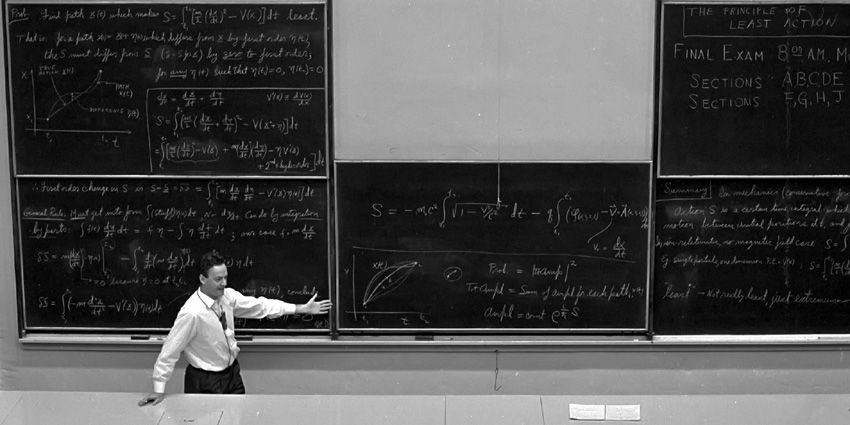
\includegraphics[width=0.7\linewidth]{fyz_fig650.jpg}
      \caption{
               (\cite[s.~707]{Feynman02})}
      \label{fyz_fig650}
    \end{figure}

    \begin{figure}[ht!] %\ref{fyz_fig651}
      \centering
      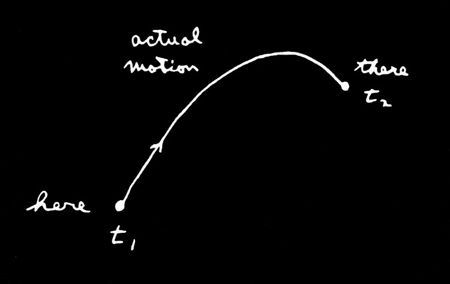
\includegraphics[width=0.7\linewidth]{fyz_fig651.jpg}
      \caption{
               (\cite[s.~707]{Feynman02})}
      \label{fyz_fig651}
    \end{figure}

    \begin{figure}[ht!] %\ref{fyz_fig652}
      \centering
      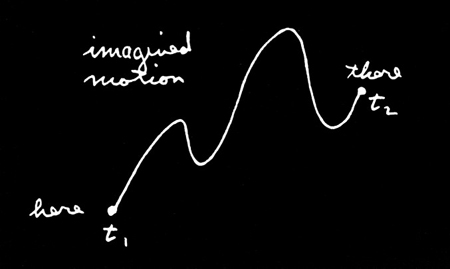
\includegraphics[width=0.7\linewidth]{fyz_fig652.jpg}
      \caption{
               (\cite[s.~707]{Feynman02})}
      \label{fyz_fig652}
    \end{figure}

    \begin{figure}[ht!] %\ref{fyz_fig653}
      \centering
      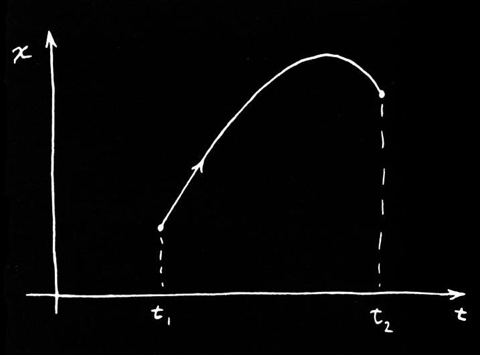
\includegraphics[width=0.7\linewidth]{fyz_fig653.jpg}
      \caption{
               (\cite[s.~707]{Feynman02})}
      \label{fyz_fig653}
    \end{figure}

    \begin{figure}[ht!] %\ref{fyz_fig654}
      \centering
      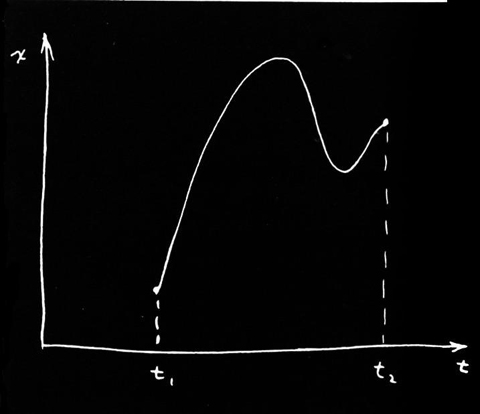
\includegraphics[width=0.7\linewidth]{fyz_fig654.jpg}
      \caption{
               (\cite[s.~707]{Feynman02})}
      \label{fyz_fig654}
    \end{figure}

    \begin{figure}[ht!] %\ref{fyz_fig655}
      \centering
      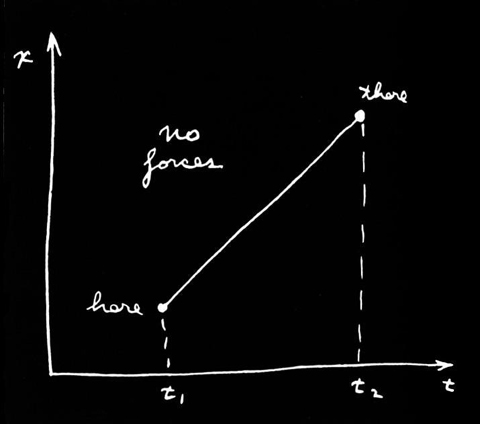
\includegraphics[width=0.7\linewidth]{fyz_fig655.jpg}
      \caption{
               (\cite[s.~707]{Feynman02})}
      \label{fyz_fig655}
    \end{figure}

    \begin{figure}[ht!] %\ref{fyz_fig656}
      \centering
      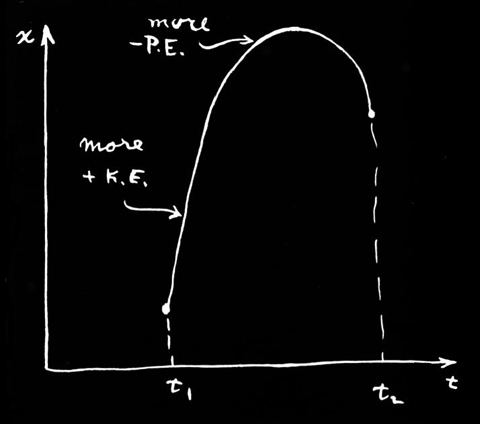
\includegraphics[width=0.7\linewidth]{fyz_fig656.jpg}
      \caption{
               (\cite[s.~707]{Feynman02})}
      \label{fyz_fig656}
    \end{figure}

    \begin{figure}[ht!] %\ref{fyz_fig657}
      \centering
      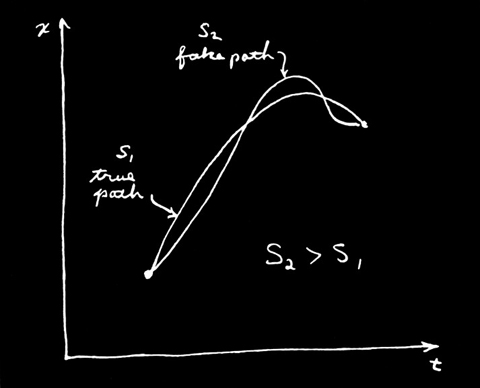
\includegraphics[width=0.7\linewidth]{fyz_fig657.jpg}
      \caption{
               (\cite[s.~707]{Feynman02})}
      \label{fyz_fig657}
    \end{figure}

    \begin{figure}[ht!] %\ref{fyz_fig658}
      \centering
      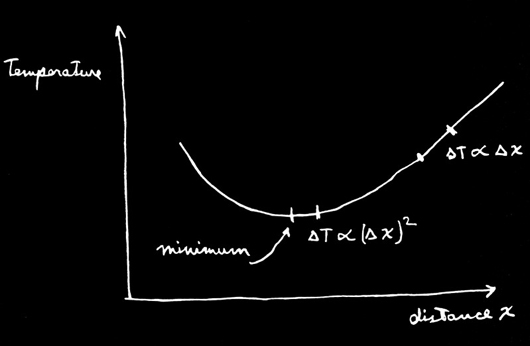
\includegraphics[width=0.7\linewidth]{fyz_fig658.jpg}
      \caption{
               (\cite[s.~707]{Feynman02})}
      \label{fyz_fig658}
    \end{figure}

    \begin{figure}[ht!] %\ref{fyz_fig659}
      \centering
      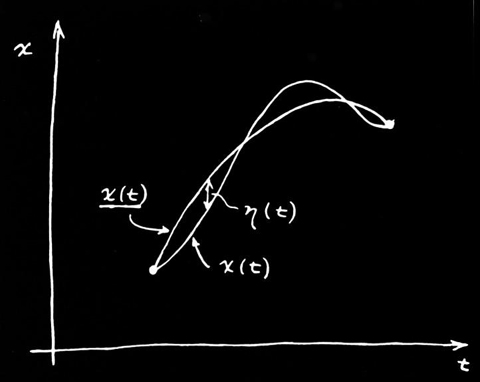
\includegraphics[width=0.7\linewidth]{fyz_fig659.jpg}
      \caption{
               (\cite[s.~707]{Feynman02})}
      \label{fyz_fig659}
    \end{figure}

    \begin{figure}[ht!] %\ref{fyz_fig660}
      \centering
      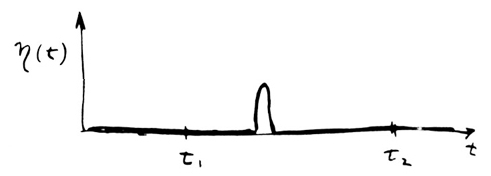
\includegraphics[width=0.7\linewidth]{fyz_fig660.jpg}
      \caption{
               (\cite[s.~707]{Feynman02})}
      \label{fyz_fig660}
    \end{figure}

    \begin{figure}[ht!] %\ref{fyz_fig661}
      \centering
      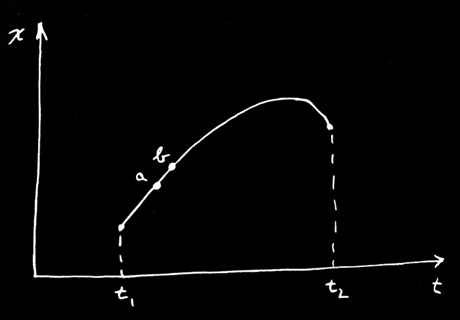
\includegraphics[width=0.7\linewidth]{fyz_fig661.jpg}
      \caption{
               (\cite[s.~707]{Feynman02})}
      \label{fyz_fig661}
    \end{figure}

    \begin{figure}[ht!] %\ref{fyz_fig662}
      \centering
      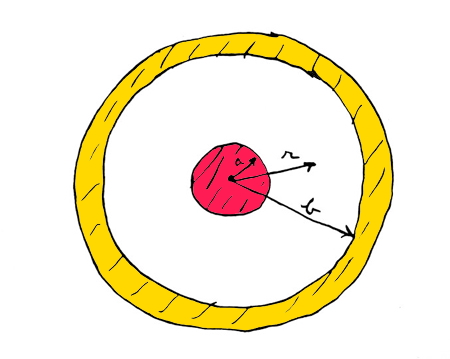
\includegraphics[width=0.7\linewidth]{fyz_fig662.jpg}
      \caption{
               (\cite[s.~707]{Feynman02})}
      \label{fyz_fig662}
    \end{figure}

} %tikzset
%---------------------------------------------------------------------------------------------------
%\printbibliography[title={Seznam literatury},heading=subbibliography]
\addcontentsline{toc}{section}{Seznam literatury}